% Chapter 1

\chapter{Título del capítulo} % Main chapter title

\label{Capitulo1} % For referencing the chapter elsewhere, use \ref{Chapter1} 

\lhead{Capítulo 1. \emph{Título del capítulo}} % This is for the header on each page - perhaps a shortened title

\newcommand{\maskalgo}{\textit{M}}
\newcommand{\NOmaskalgo}{\textit{NM}}
\newcommand{\difrelativa}{\textit{DiferenciaRelativa}}


\clearpage


\begin{table}[h]
\vspace{+5pt}
\begin{center}
    \begin{tabular}{| C{2cm} || C{2.5cm} | C{1.3cm} |  C{1.3cm} |  C{5.5cm} |}
    \hline
      \multicolumn{1}{|>{\centering\arraybackslash}m{2cm}||}{\textbf{Dataset}}
    & \multicolumn{1}{>{\centering\arraybackslash}m{2.5cm}|}{\textbf{Dataset Characteristic}} 
    & \multicolumn{1}{>{\centering\arraybackslash}m{1.3cm}|}{\textbf{\#Files}} 
    & \multicolumn{1}{>{\centering\arraybackslash}m{1.3cm}|}{\textbf{\#Types}}
    & \multicolumn{1}{>{\centering\arraybackslash}m{5.5cm}|}{\textbf{Data Types}}\\
    \hline
    \datasetirkis\ \cite{dataset:irkis, dataset:irkis2}   & Many gaps     & 7  & 1 & VWC \\\hline
    \datasetsst\ \cite{dataset:sst1}      & Many gaps     & 3  & 1 & SST \\\hline
    \datasetadcp\ \cite{dataset:sst1}     & Many gaps     & 3  & 1 & Vel \\\hline
    \datasetelnino\ \cite{dataset:elnino} & Many gaps     & 1  & 7 & \datasetelninocols \\\hline
    \datasetsolar\ \cite{dataset:solar}   & Few gaps      & 4  & 3 & \datasetsolarcols \\\hline
    \datasethail\ \cite{dataset:spc}      & No gaps       & 1  & 3 & \datasethailcols \\\hline
    \datasettornado\ \cite{dataset:spc}   & No gaps       & 1  & 2 & \datasettornadocols \\\hline
    \datasetwind\ \cite{dataset:spc}      & No gaps       & 1  & 3 & \datasetwindcols \\\hline
    \toprule[0.1mm]
    \end{tabular}
    \caption{Datasets overview. The second column indicates the characteristic of each dataset, in terms of the amount of gaps. The third column shows the number of files. The fourth and fifth columns show the number of data types and their names, respectively.}
    \label{datasets:table:overview}
\end{center}
\end{table}



En los experimentos realizados se codificaron los datasets combinando estos cuatro parámetros:
\vspace{-8pt}
\begin{itemize}
    \item 21 tipos de dato: ver tabla (\ref{tabla:resumen-de-los-datasets})
    \item 13 codificadores: 
        \begin{itemize}
            \item CoderBase
            \item CoderPCA-NM y CoderPCA-M
            \item CoderAPCA-NM y CoderAPCA-M
            \item CoderCA-NM y CoderCA-M
            \item CoderPWLH-NM y CoderPWLH-M
            \item CoderPWLHInt-NM y CoderPWLHInt-M
            \item CoderGampsLimit-NM y CoderGampsLimit-M
        \end{itemize}
    \item 8 umbrales de error: 0 (sin pérdida), y 1, 3, 5, 10, 15, 20 y 30 (con pérdida)
    \item 7 tamaños de ventana: 4, 8, 16, 32, 64, 128 y 256.
\end{itemize}

Algunas consideraciones a tener en cuenta:
\vspace{-8pt}
\begin{itemize}
    \item El codificador CoderBase solamente codifica sin pérdida e ignora el parámetro del tamaño de ventana. 
    \item Para los codificadores CoderPCA-NM y CoderPCA-M el tamaño de ventana es fijo, mientras que en el resto de los algoritmos (salvo CoderBase) el tamaño de ventana es variable y el parámetro indica su tamaño máximo.
\end{itemize}

\clearpage

Para comparar el rendimiento relativo de los algoritmos con ($\maskalgo$) y sin ($\NOmaskalgo$) máscara, utilizamos la siguiente ecuación
\vspace{-8pt}
\newcommand{\nmbits}{\NOmaskalgo_{\textit{S}}}
\newcommand{\mbits}{\maskalgo_\textit{S}}
\begin{equation}
\label{eq:diferencia-relativa}
%
 \difrelativa(\mbits, \nmbits)  =
  \begin{cases}
   100\times\frac{\nmbits - \mbits}{ \nmbits }, \quad & \text{si } \nmbits \ne \mbits, \\
   0,                   & \text{si } \nmbits = \mbits,
  \end{cases}
%  
\end{equation}
donde $\mbits$ y $\nmbits$ son los tamaños de los archivos codificados con los respectivos algoritmos. El algoritmo $\maskalgo$ logra una mejor tasa de compresión que el algoritmo $\NOmaskalgo$ cuando el resultado de la ecuación \ref{eq:diferencia-relativa} es mayor a cero. Mientras mayor sea dicho valor, mejor será el rendimiento relativo del algoritmo $\maskalgo$ respecto al algoritmo $\NOmaskalgo$.

[Se considera el dataset de manera global, tomando la ventana óptima global por algoritmo en cada caso. NOTA: para un umbral de error y modo fijo, la ventana óptima global no tiene por qué ser la misma para todos los algoritmos.]

En la tabla \ref{tabla:rendimiento-relativ-NM-M} se muestra un resumen de los resultados obtenidos al comparar el rendimiento relativo de los algoritmos $\NOmaskalgo$ y $\maskalgo$ para cada cada dataset. En la tercera y cuarta columnas aparece el porcentaje de las combinaciones <tipo de dato, codificador, umbral> con las que se obtiene la mejor tasa con cada algoritmo. En la última columna se muestra el rango en el que varía el resultado de la ecuación $\difrelativa$ para dichas combinaciones.

En los datasets que tienen muchos gaps siempre se obtienen mejores tasas al utilizar los algoritmos $\maskalgo$. En cambio, en los datasets sin gaps siempre se tiene mejor rendimiento con los algoritmos $\NOmaskalgo$. En el dataset con pocos gaps, en cada mitad de las combinaciones se obtienen mejores tasas con algoritmos diferentes.\\

\vspace{-5pt}

\begin{table}[h]
\begin{center}
    \begin{tabular}{| C{2.2cm} || C{2.5cm} | C{4.4cm} | C{3.0cm} |}
    \hline
      \multicolumn{1}{|>{\centering\arraybackslash}m{2.2cm}||}{\textbf{Dataset}} 
    & \multicolumn{1}{>{\centering\arraybackslash}m{2.5cm}|}{\textbf{Dataset Characterstic}} 
    & \multicolumn{1}{>{\centering\arraybackslash}m{4.4cm}|}{\textbf{Cases where masking outperforms non-masking variant (\%)}}
    & \multicolumn{1}{>{\centering\arraybackslash}m{3.0cm}|}{\textbf{RD (\%) Range}}\\
    \hline
    \datasetirkis   & Many gaps     & 100 & (0; 36.88]                    \\\hline
    \datasetsst     & Many gaps     & 100 & (0; \textcolor{red}{50.60}]  \\\hline
    \datasetadcp    & Many gaps     & 100 & (0; 17.35]                    \\\hline
    \datasetelnino  & Many gaps     & 100 & (0; 50.52]                    \\\hline
    \datasetsolar   & Few gaps      & 51  & [-0.25; 1.77]                 \\\hline
    \datasethail    & No gaps       & 0   & [-0.04; 0)                    \\\hline
    \datasettornado & No gaps       & 0   & [\textcolor{blue}{-0.29}; 0)   \\\hline
    \datasetwind    & No gaps       & 0   & [-0.12; 0)                    \\\hline
    \toprule[0.1mm]
    \end{tabular}
    \caption{Relative difference between the masking and non-masking variants of each algorithm. In the last column we highlight the maximum (red) and minimum (blue) values taken by RD.}
    \label{tabla:rendimiento-relativ-NM-M}
\end{center}
\end{table}

\vspace{-10pt}

Observamos que, en los casos en los que se obtienen mejores tasas con el algoritmo $\NOmaskalgo$, la diferencia relativa siempre está cerca de 0. En la figura \ref{fig:diff-tornadp} vemos que la mejor diferencia relativa a favor de $\NOmaskalgo$ se obtiene para el tipo de dato ``Longitude" del dataset NOAA-SPC-tornado, con el codificador CoderAPCA-$\NOmaskalgo$ y umbral de error 30\%. Como se observa en la tabla \ref{tabla:rendimiento-relativ-NM-M}, dicho valor es~$-0,29$.

Por otro lado, cuando se logran mejores tasas con el algoritmo $\maskalgo$ las diferencias relativas son mucho mayores, alcanzando un máximo de 50,60 para el tipo de dato ``VWC" del dataset NOAA-SST. En la figura \ref{fig:diff-noaasst} vemos que dicho resultado se obtiene con el codificador CoderPCA-$\maskalgo$ y umbral de error 30\%.

Teniendo en cuenta los resultados presentados, si quisiéramos codificar un dataset que a priori supiéramos tiene muchos gaps, obviamente nos convendría utilizar el algoritmo $\maskalgo$. Pero aún si el dataset no tuviera gaps, la diferencia de rendimiento a favor del algoritmo $\NOmaskalgo$ sería despreciable. Como el algoritmo $\maskalgo$ es más robusto y funciona mejor en general, en las próximas secciones nos vamos a enfocar en su estudio.




\begin{sidewaysfigure}
  \centering
    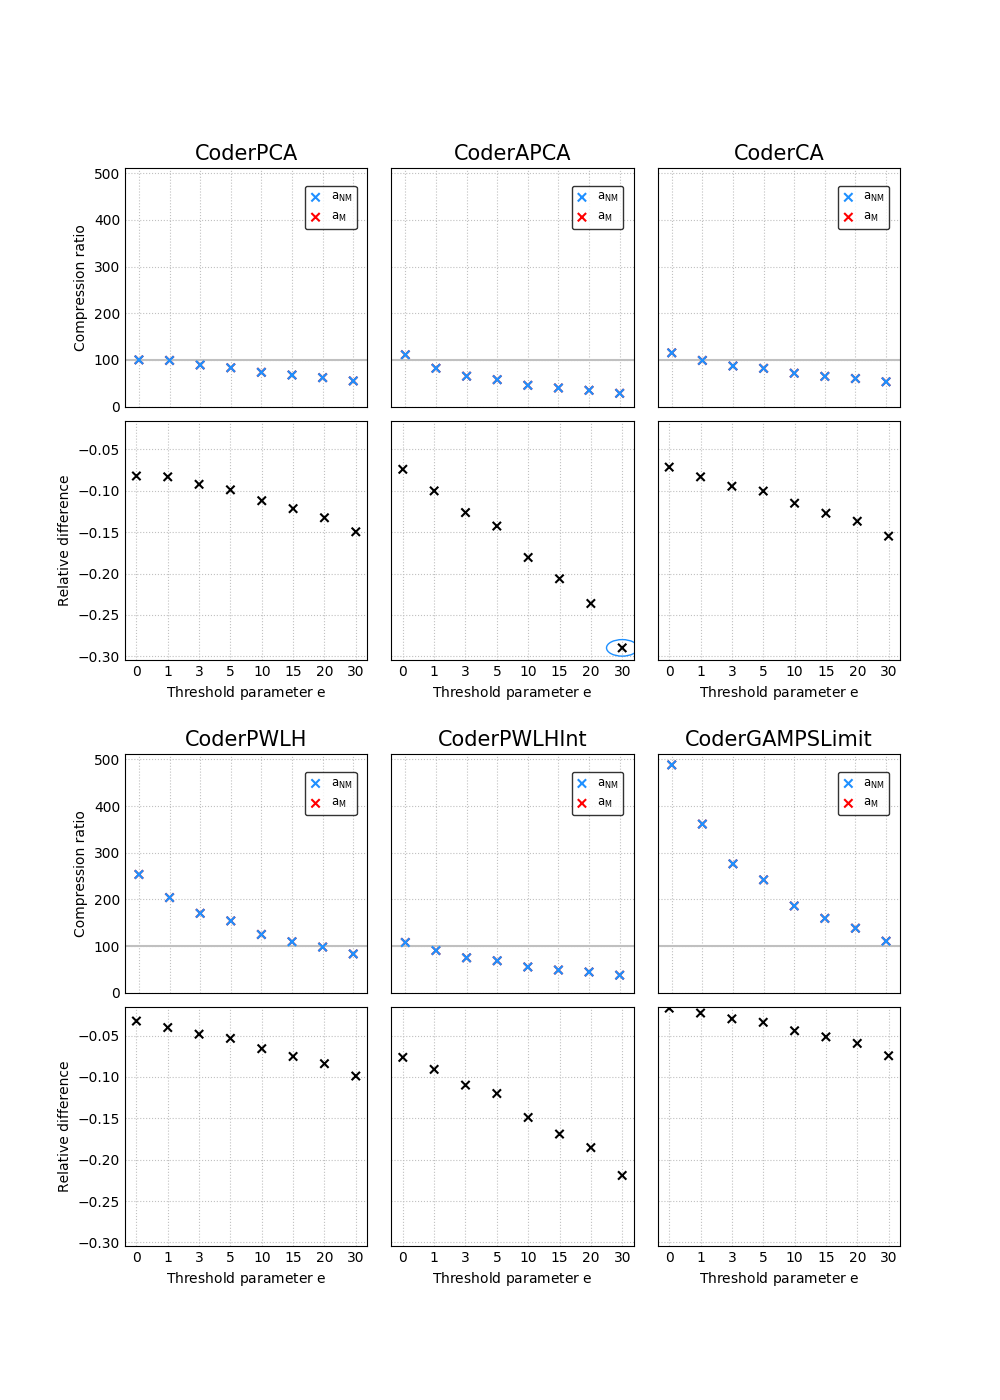
\includegraphics[scale=0.47]{chapter1/7-NOAA-SPC-tornado-2.png}
    \caption{Tasa de compresión y Diferencia relativa para las distintas combinaciones\\ <codificador, umbral> para el tipo de dato ``Longitude" del dataset NOAA-SPC-tornado.}
  \label{fig:diff-tornadp}
  \vspace{20pt}
    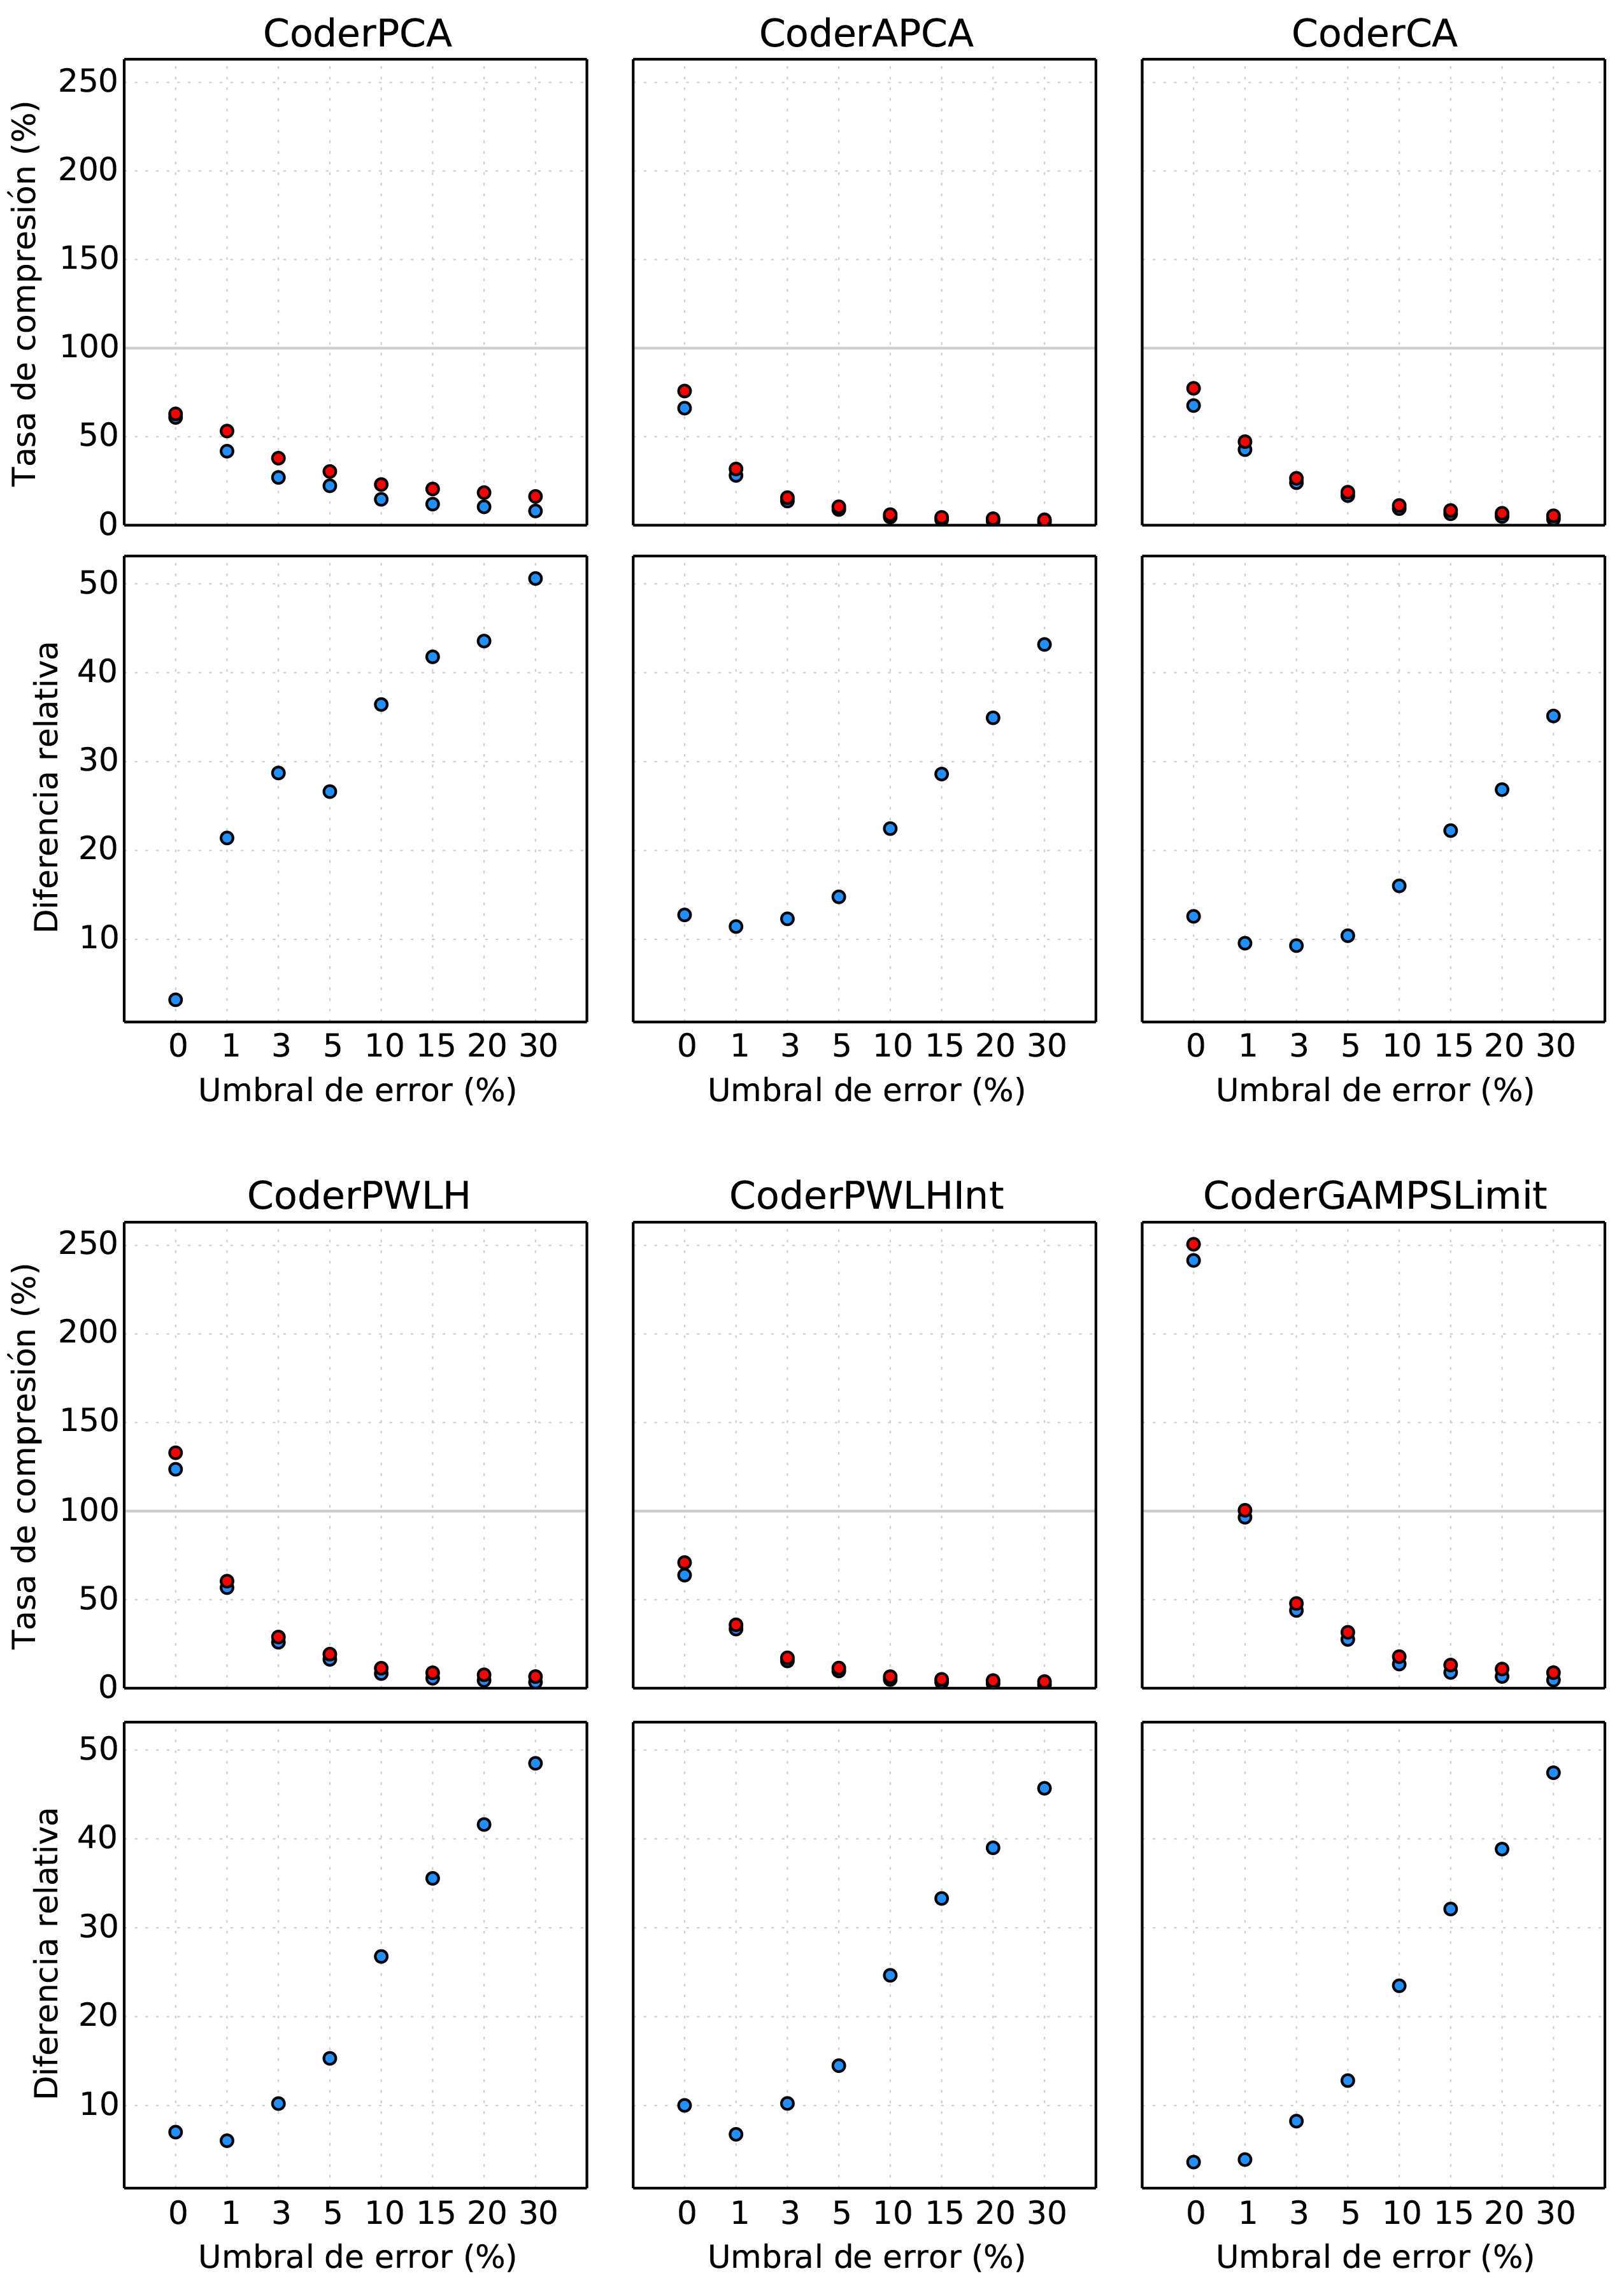
\includegraphics[scale=0.47]{chapter1/Global-2-NOAA-SST.png}
    \caption{Tasa de compresión y Diferencia relativa para las distintas combinaciones\\ <codificador, umbral> para el tipo de dato ``VWC" del dataset NOAA-SST.}
  \label{fig:diff-noaasst}
  \vspace{+25pt}
\end{sidewaysfigure}



\clearpage

HECHO INFORME:

- Elegir nomenclatura para los dos distintos modos de ejecución => CoderPCA-NM (sin máscara) y CoderPCA-M (con máscara).

- Realizar un análisis cuantitativo para saber qué tanto mejor comprime el modo MM=0 en los pocos casos en los que funciona mejor que el modo MM=3. Vimos que esos casos se dan en los datasets con pocos o ningún gap, y la diferencia en las tasas de compresión es mínima. En cambio, cuando hay gaps en los datasets, la diferencia relativa de rendimiento a favor del modo MM=3 es mayor. Escribir un párrafo con dicho análisis, incluyendo alguna gráfica como ejemplo.

- Agregar tabla con resumen de los datasets - ver AVANCES / DUDAS (13)

% \clearpage
\vspace{+20pt}

TODO INFORME:

- Poner las gráficas horizontales, 3 arriba y 3 abajo.

- Vimos que en los datasets sin gaps, en general para todas las combinaciones <tipo de dato, algoritmo> la diferencia relativa no crece al aumentar el umbral de error. Escribir un párrafo explicando el por qué de este comportamiento.

- Mencionar experimentos ventana local vs ventana global. (ver minuta de la reunión del lunes 10/06/2019).

- Mencionar relación de compromiso entre el umbral y la tasa de compresión: al aumentar el umbral mejor la tasa de compresión (lógico).

- Mencionar que CoderSlideFilter no tiene en cuenta el parámetro con el tamaño máximo de la ventana.

- Agregar tabla con resumen de los algoritmos.

- Subir todo el material complementario en un link (después referirlo en el informe)

\clearpage

TODO CÓDIGO:

- Para los experimentos sin máscara no se están considerando los datos para los algoritmos CoderFractalRestampling y CoderSlideFilter.

- Agregar tests para MM=3.

- Al ejecutar los algoritmos GAMPS/GAMPSLimit sobre el dataset de "El Niño" (546 columnas) tengo problemas de memoria en Ubuntu, pero no en la Mac.

- Universalizar algoritmo

- Modificar GAMPS/GAMPSLimit para que utilice floats (4 bytes) en vez de doubles (8 bytes). De todas maneras, no creo que esto cambie los resultados de manera significativa, ya que aun si la cantidad de bits utilizados al codificar con GAMPS/GAMPSLimit fuera la mitad, en ningún caso superaría la tasa obtenida con el mejor codificador.